\documentclass[tikz,border=2mm]{standalone}
\usepackage[T1]{fontenc}
\usepackage[swedish,english]{babel}
\usepackage{tikz}
\usetikzlibrary{arrows,positioning}
\usepackage{pgfplots}
\usepackage{amsmath,mathtools}
\usepgfplotslibrary{fillbetween}
\begin{document}
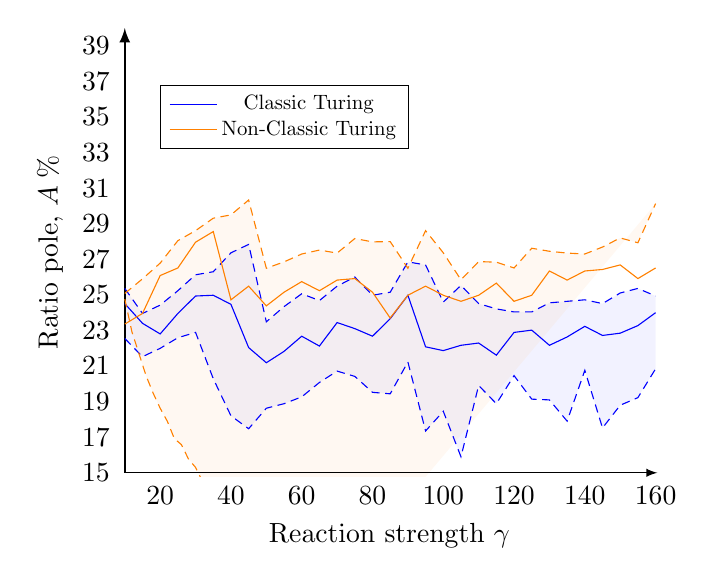
\begin{tikzpicture}
\begin{axis}[
    %hide axis,
    %axis lines* = left,
    %axis lines=left, xtick=\empty, ytick=\empty.
    axis line style={draw=none},
    tick style={draw=none},
    xticklabel style={yshift=-0.1mm},
    xmin = 8.5,
   xmax = 161,
    ymin = 14.8,
    ymax = 40,
    %grid=both,
    %xtick = {1,0.95,...,0.6},
    ytick = {15,17,...,100},    
    %xticklabels = {{zero},$\alpha$,$\varphi$},
   %xlabel style={at={(axis cs:0.61,7)},anchor=east,align=center},
    %ylabel style={at={(axis cs:1.00,35)},anchor=north,rotate=0},
	xlabel = {Reaction strength $\gamma$},
        ylabel = {Ratio pole, $A\;\%$},
    legend style={at={(axis cs:20,35)},anchor=west,cells={align=center},nodes={scale=0.75}},
    %x dir=reverse
    %legend entries = {Decreasing the inactivation rate $k_{-2}$}
]
%-------------------------------------------------------------------------------------------------
% AXES
\draw[->,-latex, thick] (axis cs: 10,15) -- (axis cs: 10,40); % y-axis
\draw[->,-latex] (axis cs: 10,15) -- (axis cs: 160.5,15); % x-axis
%-------------------------------------------------------------------------------------------------
%-------------------------------------------------------------------------------------------------
% Classical 
%-------------------------------------------------------------------------------------------------
\addplot[forget plot,densely dashed,color=blue,name path=UpratioPoleClassical] coordinates {
		(10.0000	,	25.3623	)
		(15.0000	,	23.9557	)
		(20.0000	,	24.4246	)
		(25.0000	,	25.2344	)
		(30.0000	,	26.1296	)
		(35.0000	,	26.3001	)
		(40.0000	,	27.3657	)
		(45.0000	,	27.8346	)
		(50.0000	,	23.4868	)
		(55.0000	,	24.3393	)
		(60.0000	,	25.0639	)
		(65.0000	,	24.6803	)
		(70.0000	,	25.4902	)
		(75.0000	,	26.0017	)
		(80.0000	,	24.9787	)
		(85.0000	,	25.1492	)
		(90.0000	,	26.8542	)
		(95.0000	,	26.6837	)
		(100.0000	,	24.5951	)
		(105.0000	,	25.5328	)
		(110.0000	,	24.5098	)
		(115.0000	,	24.2114	)
		(120.0000	,	24.0409	)
		(125.0000	,	24.0409	)
		(130.0000	,	24.5524	)
		(135.0000	,	24.6377	)
		(140.0000	,	24.7229	)
		(145.0000	,	24.5098	)
		(150.0000	,	25.1066	)
		(155.0000	,	25.3623	)
		(160.0000	,	24.9361	)
};

\addplot[color=blue] coordinates {
		(10.0000	,	24.5098	)
		(15.0000	,	23.4015	)
		(20.0000	,	22.8048	)
		(25.0000	,	23.9557	)
		(30.0000	,	24.9361	)
		(35.0000	,	24.9787	)
		(40.0000	,	24.4672	)
		(45.0000	,	22.0375	)
		(50.0000	,	21.1850	)
		(55.0000	,	21.8244	)
		(60.0000	,	22.6769	)
		(65.0000	,	22.1228	)
		(70.0000	,	23.4442	)
		(75.0000	,	23.1032	)
		(80.0000	,	22.6769	)
		(85.0000	,	23.6573	)
		(90.0000	,	24.9787	)
		(95.0000	,	22.0801	)
		(100.0000	,	21.8670	)
		(105.0000	,	22.1654	)
		(110.0000	,	22.2933	)
		(115.0000	,	21.6113	)
		(120.0000	,	22.8900	)
		(125.0000	,	23.0179	)
		(130.0000	,	22.1654	)
		(135.0000	,	22.6343	)
		(140.0000	,	23.2310	)
		(145.0000	,	22.7195	)
		(150.0000	,	22.8474	)
		(155.0000	,	23.2737	)
		(160.0000	,	23.9983	)
};

\addplot[forget plot,densely dashed,color=blue,name path=DownratioPoleClassical] coordinates {
		(10.0000	,	22.5490	)
		(15.0000	,	21.5260	)
		(20.0000	,	21.9949	)
		(25.0000	,	22.5916	)
		(30.0000	,	22.8900	)
		(35.0000	,	20.2899	)
		(40.0000	,	18.2012	)
		(45.0000	,	17.4766	)
		(50.0000	,	18.6275	)
		(55.0000	,	18.8832	)
		(60.0000	,	19.2668	)
		(65.0000	,	20.0767	)
		(70.0000	,	20.7161	)
		(75.0000	,	20.4177	)
		(80.0000	,	19.5226	)
		(85.0000	,	19.4373	)
		(90.0000	,	21.2276	)
		(95.0000	,	17.3487	)
		(100.0000	,	18.4569	)
		(105.0000	,	15.8994	)
		(110.0000	,	19.9062	)
		(115.0000	,	18.8832	)
		(120.0000	,	20.4604	)
		(125.0000	,	19.1390	)
		(130.0000	,	19.0963	)
		(135.0000	,	17.9028	)
		(140.0000	,	20.7587	)
		(145.0000	,	17.5192	)
		(150.0000	,	18.7980	)
		(155.0000	,	19.2242	)
		(160.0000	,	20.8440	)
};
\addplot[blue!50,opacity=0.1,forget plot] fill between[of=UpratioPoleClassical and DownratioPoleClassical];

\addlegendentry{Classic Turing}% Add to legend
%-------------------------------------------------------------------------------------------------
% Non-classical
%-------------------------------------------------------------------------------------------------
\addplot[forget plot,densely dashed,color=orange,name path=UpratioPoleNonClassical] coordinates {
		(10.0000	,	25.0810	)
		(15.0000	,	25.8994	)
		(20.0000	,	26.7860	)
		(25.0000	,	28.0477	)
		(30.0000	,	28.6104	)
		(35.0000	,	29.3095	)
		(40.0000	,	29.4970	)
		(45.0000	,	30.3325	)
		(50.0000	,	26.4962	)
		(55.0000	,	26.8542	)
		(60.0000	,	27.2975	)
		(65.0000	,	27.5192	)
		(70.0000	,	27.3487	)
		(75.0000	,	28.1671	)
		(80.0000	,	27.9795	)
		(85.0000	,	27.9966	)
		(90.0000	,	26.4962	)
		(95.0000	,	28.6104	)
		(100.0000	,	27.3657	)
		(105.0000	,	25.8483	)
		(110.0000	,	26.8713	)
		(115.0000	,	26.8372	)
		(120.0000	,	26.5132	)
		(125.0000	,	27.6215	)
		(130.0000	,	27.4510	)
		(135.0000	,	27.3487	)
		(140.0000	,	27.2975	)
		(145.0000	,	27.6897	)
		(150.0000	,	28.2012	)
		(155.0000	,	27.9284	)
		(160.0000	,	30.1279	)
};

\addplot[color=orange] coordinates {
		(10.0000	,	23.3589	)
		(15.0000	,	23.9557	)
		(20.0000	,	26.0870	)
		(25.0000	,	26.5132	)
		(30.0000	,	27.9625	)
		(35.0000	,	28.5592	)
		(40.0000	,	24.7229	)
		(45.0000	,	25.4902	)
		(50.0000	,	24.3819	)
		(55.0000	,	25.1492	)
		(60.0000	,	25.7460	)
		(65.0000	,	25.2344	)
		(70.0000	,	25.8312	)
		(75.0000	,	25.9165	)
		(80.0000	,	25.1492	)
		(85.0000	,	23.6999	)
		(90.0000	,	24.9787	)
		(95.0000	,	25.4902	)
		(100.0000	,	24.9787	)
		(105.0000	,	24.6377	)
		(110.0000	,	24.9787	)
		(115.0000	,	25.6607	)
		(120.0000	,	24.6377	)
		(125.0000	,	24.9787	)
		(130.0000	,	26.3427	)
		(135.0000	,	25.8312	)
		(140.0000	,	26.3427	)
		(145.0000	,	26.4280	)
		(150.0000	,	26.6837	)
		(155.0000	,	25.9165	)
		(160.0000	,	26.5132	)
};

\addplot[forget plot,densely dashed,color=orange,name path=DownratioPoleNonClassical] coordinates {
		(10.0000	,	24.7656	)
		(12.0000	,	22.9327	)
		(14.0000	,	21.6965	)
		(16.0000	,	20.4604	)
		(18.0000	,	19.4800	)
		(20.0000	,	18.6275	)
		(22.0000	,	17.9028	)
		(24.0000	,	16.9224	)
		(26.0000	,	16.5814	)
		(28.0000	,	15.7715	)
		(30.0000	,	15.3026	)
		(32.0000	,	14.4928	)
		(34.0000	,	14.1091	)
		(36.0000	,	13.8960	)
		(38.0000	,	12.8730	)
		(40.0000	,	12.7025	)
		(42.0000	,	12.3188	)
		(44.0000	,	11.8926	)
		(46.0000	,	11.2958	)
		(48.0000	,	11.4237	)
		(50.0000	,	11.5942	)
		(52.0000	,	10.4433	)
		(54.0000	,	10.1023	)
		(56.0000	,	10.3154	)
		(58.0000	,	10.1876	)
		(60.0000	,	9.6760	)
		(62.0000	,	9.4629	)
		(64.0000	,	9.2072	)
		(66.0000	,	9.1645	)
		(68.0000	,	8.9940	)
		(70.0000	,	8.8662	)
};
\addplot[orange!50,opacity=0.1,forget plot] fill between[of=UpratioPoleNonClassical and DownratioPoleNonClassical];

\addlegendentry{Non-Classic Turing}% Add to legend
\end{axis}

\end{tikzpicture}



\end{document}
